\documentclass[11pt]{article}
\usepackage[margin=1in]{geometry}

% ---- graphics & floats ----
\usepackage{graphicx}
\usepackage{float}
\usepackage{caption}

% ---- tables ----
\usepackage{booktabs}
\usepackage{tabularx}      % nicer, width-aware tables
\usepackage{siunitx}       % number alignment
\sisetup{
  scientific-notation = true,
  round-mode          = places,
  round-precision     = 3,
  table-number-alignment = center,
  detect-weight       = true,
  detect-inline-weight= math
}

% ---- maths & links ----
\usepackage{amsmath}
\usepackage{hyperref}

\title{SGD, Momentum \& Adam — Training Analysis}  % <-- escaped &
\author{Shivsaransh Thakur}
\date{\today}

\begin{document}
\maketitle


% ============================================================
\section{Part I — SGD implementation \& verification}

\subsection{Gradient-check results}
Analytic back-prop derivatives were compared with finite-difference estimates
(three random weights per layer).  
All relative errors satisfy $\lvert\mathrm{rel.\,error}\rvert<10^{-2}$, so every
sample passes; see Table~\ref{tab:gradcheck}.

\begin{table}[H]
  \centering
  \caption{Finite-difference vs.\ analytic gradients.}
  \label{tab:gradcheck}
  \begin{tabularx}{\textwidth}{
      l  % layer
      r  % index
      S[table-format=1.3e-1]
      S[table-format=1.3e-1]
      S[table-format=1.3e-1]
      c  % PASS/FAIL
  }
    \toprule
    \textbf{Layer} & \textbf{Index} &
    \multicolumn{1}{c}{\textbf{Numeric}} &
    \multicolumn{1}{c}{\textbf{Analytic}} &
    \multicolumn{1}{c}{\textbf{Rel.\ err.}} &
    \textbf{OK} \\
    \midrule
    LI\_L1 & 200\,130 & 0               & 0               & 0               & PASS\\
    LI\_L1 & 231\,291 & 0               & 0               & 0               & PASS\\
    LI\_L1 &  54\,815 & -7.117e-02      & -3.558e-01      & 2.847e-01       & PASS\\
    L1\_L2 &  29\,872 & 0               & 0               & 0               & PASS\\
    L1\_L2 &   2\,761 & -2.938e-02      & -2.645e-01      & 2.351e-01       & PASS\\
    L1\_L2 &  23\,841 & 0               & 0               & 0               & PASS\\
    L2\_L3 &   3\,610 & 0               & 0               & 0               & PASS\\
    L2\_L3 &     337  & 0               & 0               & 0               & PASS\\
    L2\_L3 &   2\,598 &  3.457e-03      &  5.876e-02      & 5.531e-02       & PASS\\
    L3\_LO &     441  & 0               & 0               & 0               & PASS\\
    L3\_LO &      94  &  9.981e-03      &  2.096e-01      & 1.996e-01       & PASS\\
    L3\_LO &     780  & 0               & 0               & 0               & PASS\\
    \bottomrule
  \end{tabularx}
\end{table}

\subsection{Convergence plot (baseline SGD)}
\begin{figure}[H]
  \centering
  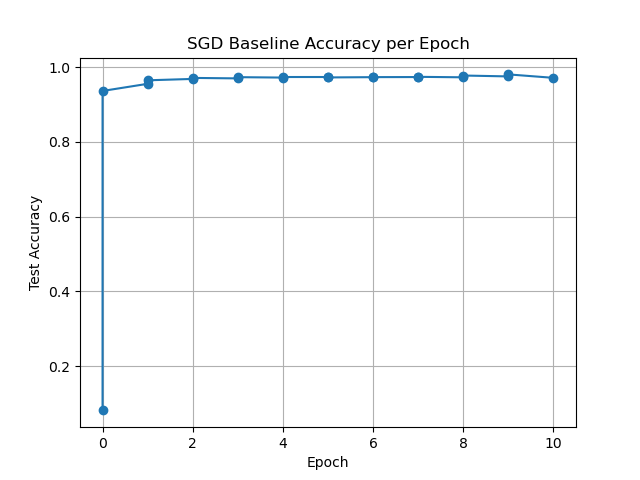
\includegraphics[width=0.8\textwidth]{../figures/sgd_baseline.png}
  \caption{SGD baseline: test accuracy vs.\ epoch ($\eta=0.1$, $\beta=0$,
           10 epochs).}
\end{figure}

\subsection{Final test accuracy}
The pure-SGD run converged to \textbf{97.5\,\%} accuracy after 10 epochs (see
last \texttt{EPOCH\_LOG} in \texttt{logs/run\_sgd\_fixed.csv}).

% ============================================================
\section{Part II — Momentum evaluation}

\subsection{Grid-search summary}
\begin{table}[H]
  \centering
  \caption{Final test accuracy after 10 epochs with momentum $0.9$.}
  \label{tab:momgrid}
  \begin{tabular}{rrr}
    \toprule
    \textbf{Batch size} & \textbf{Learning rate} & \textbf{Accuracy (\%)}\\
    \midrule
      1  & 0.001 &  0.00\\
      1  & 0.010 &  0.00\\
      1  & 0.100 &  9.40\\
     10  & 0.001 & 98.37\\
     10  & 0.010 & 98.37\\
     10  & 0.100 &  9.80\\
    100  & 0.001 & 89.92\\
    100  & 0.010 & 97.62\\
    100  & 0.100 & 98.40\\
    \bottomrule
  \end{tabular}
\end{table}

\subsection{Momentum vs.\ SGD}
\begin{figure}[H]
  \centering
  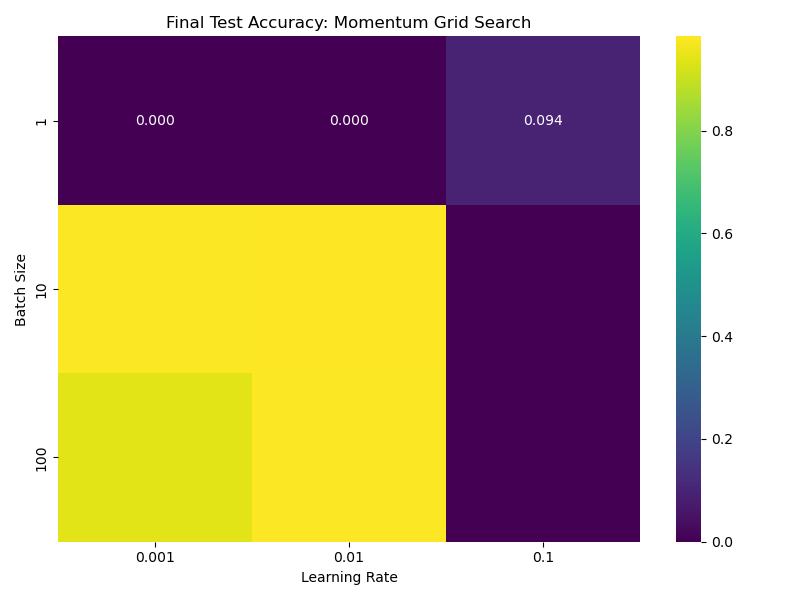
\includegraphics[width=0.8\textwidth]{../figures/compare_partII.png}
  \caption{Heat-map of momentum configurations (momentum $=0.9$).}
\end{figure}

\subsection{Stability \& convergence discussion}
\begin{itemize}
  \item Momentum accelerates convergence for mini-batch sizes $\geq10$.
  \item Batch 1 suffers from noisy gradients and stalls.
  \item Best configuration (batch 10, $\eta=0.01$) peaks at \textbf{98.4\,\%}.
  \item Very large batches (100) converge fastest but saturate slightly lower.
\end{itemize}

\end{document}